% % % % % % % % % % % % % % % % % % % % % % % % % % % % % % % % % % % % % % % % % % % %
%                                                                                     %
% Short Sectioned Assignment LaTeX Template Version 1.0 (5/5/12)                      %
% This template has been downloaded from: http://www.LaTeXTemplates.com               %
%                                                                                     %
% Original author:  Frits Wenneker (http://www.howtotex.com)                          %
%                                                                                     %
% Modified by: Fco Javier Sueza Rodríguez (fcosueza@disroot.org)                      %
%                                                                                     %
% Changes:                                                                            %
%	    - Custom Chapters, Sections and Subsections (titlesec package)                %
%           - Document type scrbook (oneside)                                         %
%           - Use babel-lang-spanish package and marvosym                             %
%           - Use hyperref, enumitem, tcolorbox and glossaries packages               %
%           - Use Time New Roman (mathptmx), Helvetic and Courier fonts               %
%                                                                                     %
% License: CC BY-NC-SA 3.0 (http://creativecommons.org/licenses/by-nc-sa/3.0/)        %
%                                                                                     %
% % % % % % % % % % % % % % % % % % % % % % % % % % % % % % % % % % % % % % % % % % % %

%-----------------------------------------------%
%	              Packages                  %
%-----------------------------------------------%

\documentclass[paper=a4, fontsize=11pt, oneside]{scrbook}

% ---- Text Input/Output ----- %

\usepackage[T1]{fontenc}
\usepackage[utf8]{inputenc}
\usepackage{mathptmx}
\usepackage[scaled=.92]{helvet}
\usepackage{courier}
\usepackage[indent=12pt]{parskip}

\usepackage{geometry}
\geometry{verbose,tmargin=3cm,bmargin=3cm,lmargin=2.6cm,rmargin=2.6cm}

% ---- Language ----- %

\usepackage[spanish]{babel}
\usepackage{marvosym}

% ---- Another packages ---- %

\usepackage{amsmath,amsfonts,amsthm}
\usepackage{graphics,graphicx}
\usepackage{titlesec}
\usepackage{fancyhdr}
\usepackage{tcolorbox}
\usepackage{hyperref}
\usepackage{enumitem}
\usepackage[automake]{glossaries}

%--------------------------------------------------------------------%
%                      Customizing Document                          %
%--------------------------------------------------------------------%


% ----------- Custom Chapters, Sections and Subsections -------------- %

\titleformat{\chapter}[display]
			{\bfseries\Huge}
			{Tema \ \thechapter} {0.5ex}
			{\vspace{1ex}\centering}

\titleformat{\section}[hang]
			{\bfseries\Large}
			{\thesection}{0.5em}{}

\titleformat{\subsection}[hang]
			{\bfseries\large}
			{\thesubsection}{0.5em}{}

\titleformat{\subsubsection}[hang]
			{\bfseries\large}
			{\thesubsubsection}{0.5em}{}

\hypersetup{
    colorlinks=true,
    linkcolor=black,
    urlcolor=magenta
}

% ------------------- Custom heaaders and footers ------------------- %

\pagestyle{fancyplain}

\fancyhead[]{}
\fancyfoot[L]{}
\fancyfoot[C]{}
\fancyfoot[R]{\thepage}

\renewcommand{\headrulewidth}{0pt} % Remove header underlines
\renewcommand{\footrulewidth}{0pt} % Remove footer underlines

\setlength{\headheight}{13.6pt} % Customize the height of the header

% --------- Numbering equations, figures and tables ----------------- %

\numberwithin{equation}{section} % Number equations within sections
\numberwithin{figure}{section} % Number figures within sections
\numberwithin{table}{section} % Number tables within sections

% ------------------------ New Commands ----------------------------- %

\newcommand{\horrule}[1]{\rule{\linewidth}{#1}} % Create horizontal rule command


%----------------------------------------------------------------------------------------
%	TÍTULO Y DATOS DEL ALUMNO
%----------------------------------------------------------------------------------------

\title{
\vspace{10ex}
\normalfont \normalsize
\Huge \textbf{Tarea 1: Conociendo Mi Equipo}
}
\author{Francisco Javier Sueza Rodríguez}
\date{\normalsize\today}

%----------------------------------------------------------------------------------------
%                                     DOCUMENTO
%----------------------------------------------------------------------------------------
\begin{document}

\maketitle

\thispagestyle{empty}

\vspace{75ex}

\begin{center}
    \begin{tabular}{l l}
        \textbf{Centro}: & IES Aguadulce \\
        \textbf{Ciclo Formativo}: & Desarrollo Aplicaciones Web (Distancia)\\
        \textbf{Asignatura}: & Sistemas Informáticos\\
        \textbf{Tema}: & Tema 1 -  Hardware de un Sistema Informático\\
    \end{tabular}
\end{center}

\newpage

%\tableofcontents

%\vspace{10ex}

%\listoffigures

%\newpage

\section{Caso Práctico}
José Manuel quiere montar un ordenador para su hermana pequeña, principalmente para jugar a videojuegos modernos y poder realizar tareas que requieran cierta potencia de computación, como la elaboración de contenidos audiovisuales; pero José Manuel no tiene muchos conocimientos de hardware. Ada le ha sugerido que pida ayuda a Juan y a María para que le enseñen los conceptos básicos sobre hardware.

José Manuel hace lo que Ada le sugiere, y Juan y María deciden empezar por enseñar a José Manuel a analizar los componentes de su propio equipo, para que vaya familiarizándose con los mismos.

\section{Actividades}
En esta sección se incluyen todas las actividades, divididas en subsecciones con su correspondiente descripción y su solución.

\subsection{Actividad 1: Resumen de Hardware}
Descarga y ejecuta el programa gratuito HWiNFO en tu equipo (se recomienda la versión "portable" ya que no requiere instalación). Una vez dentro, incluye en el documento de la tarea lo siguiente:

\begin{itemize}
    \item Una captura de la ventana "resumen del sistema" (consultar el ejemplo de solución en caso de duda), donde se resumen las principales características del equipo. En esta captura señala de manera clara (un recuadro, un subrayado, etc.) los siguientes datos:

    \begin{itemize}
        \item El modelo de la placa base y su chipset.
        \item El modelo de la CPU.
        \item El modelo de la GPU.
        \item Tipo, cantidad y velocidad de la memoria RAM.
        \item Las opciones de virtualización de la CPU. Esto aparece en el apartado "características", con el nombre "VMX" o "VT-x" si tu procesador Intel, o "AMD-V" o "SVM" si tu procesador es AMD. En caso de que dicha opción aparezca en rojo en lugar de verde, debes entrar en la BIOS/UEFI de tu equipo y habilitar las opciones de virtualización de tu procesador (esta opción puede tener distintos nombres según la placa base). Esto es necesario de cara a futuras tareas.
    \end{itemize}

    \item A continuación, copia y pega el texto generado en el "resumen para portapapeles" (Reporte > Resumen para portapapeles).
\end{itemize}

Si usas un sistema operativo GNU/Linux puedes utilizar otros programas como "hardinfo" o "CPU-X". En el caso de equipos Mac puedes usar "menú Apple > Acerca de este Mac". En estos casos intenta recopilar la información básica de: CPU, placa base, chipset, memoria RAM, gráficos, unidades de almacenamiento, sonido, red y sistema operativo (una línea por cada componente).

\subsubsection{Solución}
Se ha usado el software \textbf{HWiNFO} para obtener la información sobre el hardware. El model del ordenador es un portátil \textbf{HP-15s-eq0003ns}. En la siguiente figura, se muestra la captura de pantalla pedida con la información sobre el hardware.

\begin{figure}[ht]
    \centering
    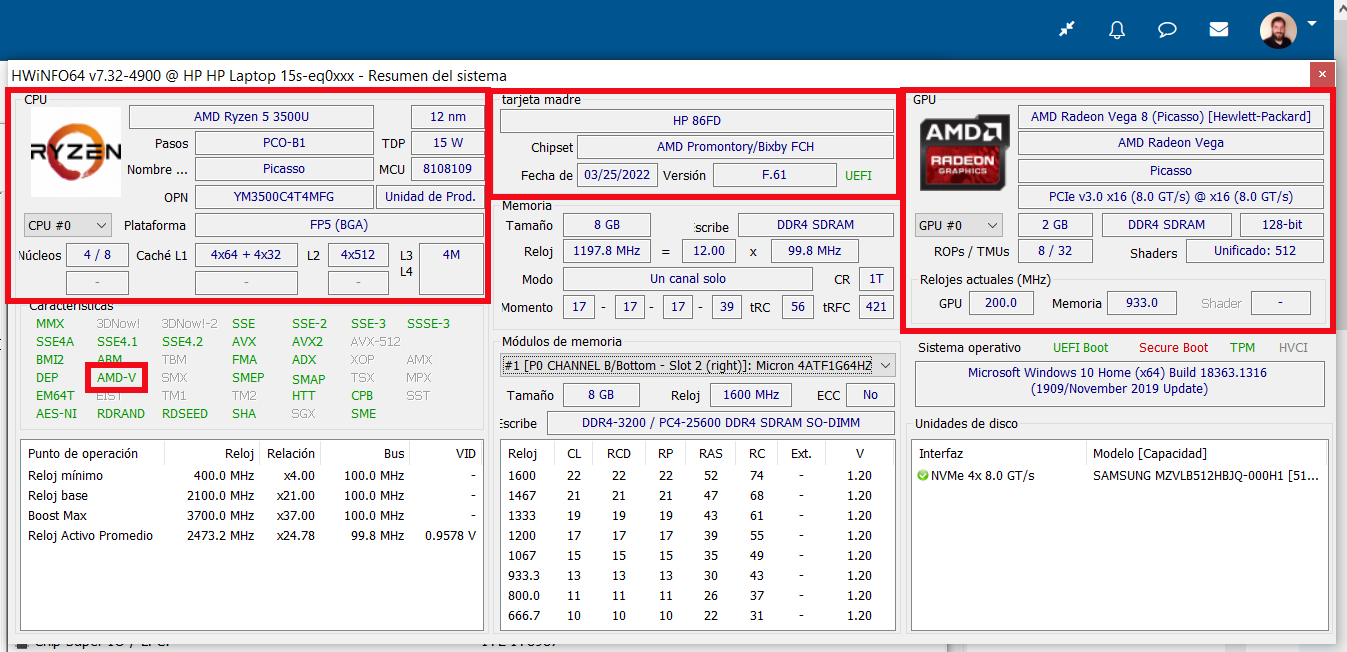
\includegraphics[scale=0.54]{info-sistema.png}
    \caption{Información hardware de HWiNFO}
\end{figure}

A continuación vemos el informe generado por HWiNfo usando la opción ``\textbf{Resumen para portapapeles}''.

\begin{figure}[ht]
    \begin{tcolorbox}[sharp corners, colback=yellow!30, colframe=white!20]
\begin{center}
    \begin{tabular}{p{6em} p{31em}}
        Computer:   &  HP HP Laptop 15s-eq0xxx \\
        CPU:        &  AMD Ryzen 5 3500U (Picasso, PCO-B1) 2100 MHz (21.00x100.0) @ 1834 MHz (18.38x99.8) \\
        Motherboard:&  HP 86FD  \\
        BIOS:       &  F.61, 03/25/2022 \\
        Chipset:    &  AMD Promontory/Bixby FCH \\
        Memory:     &  8192 MBytes @ 1197 MHz, 17-17-17-39 - 8192 MB PC25600 DDR4 SDRAM - Micro 4ATF1G64HZ-3G2E1 \\
        Graphics:   &  AMD Radeon Vega 8 (Picasso) [Hewlett-Packard] AMD Radeon Vega, 2048 MB DDR4 SDRAM \\
        Drive:      &  SAMSUNG MZVLB512HBJQ-000H1, 500.1 GB, NVMe \\
        Sound:      &  ATI/AMD Display HD Audio Controller \\
        Sound:      &  AMD Zen - Audio Processor - HD Audio Controller \\
        Network:    &  RealTek Semiconductor, Device ID: C821 \\
        OS:         &  Microsoft Windows 10 Home (x64) Build 18363.1316 (1909/November 2019 Update) \\
    \end{tabular}
\end{center}
    \end{tcolorbox}
    \caption{Reporte para portapapeles de HWiNFO}
\end{figure}

\subsection{Actvidad 2}
Utilizando como base la información que has obtenido en la actividad 1, busca la siguiente información detallada, bien en las páginas web oficiales de los fabricantes o utilizando software gratuito como HWiNFO, CPU-Z, GPU-Z, etc.:

\begin{itemize}
    \item De la CPU:
    \begin{itemize}
        \item Fabricante.
        \item Modelo.
        \item Fecha de salida al mercado.
        \item Número de núcleos y subprocesos (cores/threads)
        \item Velocidad base en GHz, si la tiene
        \item Velocidad turbo o boost en GHz, si la tiene.
        \item Tamaño de caché.
        \item Tamaño del proceso de fabricación (litografía) en "nm".
        \item  TDP en vatios.
    \end{itemize}
    \item Del adaptador gráfico:
    \begin{itemize}
        \item Indica si es una iGPU (GPU integrada en el procesador o chipset) o una GPU dedicada (tarjeta gráfica no integrada). Si tu equipo tiene ambos, elige la GPU dedicada.
        \item Fabricante del chip gráfico (Nvidia, AMD, Intel).
        \item Chip gráfico de la tarjeta (mirar ejemplo de solución).
        \item Modelo exacto.
        \item Cantidad y tipo de memoria VRAM (RAM de vídeo).
    \end{itemize}
\end{itemize}

\subsubsection{Solución}

En primer lugar se va a mostrar la información relativa al procesador, en este caso un \textbf{Ryzen 5 3500U}, en la siguiente tabla. La información ha sido obtenida de la página oficial de AMD. \cite{amd01}:

\begin{figure}[ht]
    \centering

    \setlength{\tabcolsep}{10pt}
    \renewcommand{\arraystretch}{1.5}

    \begin{tabular}{| p{10em} | p{15em} |}
        \hline
        \textbf{Fabricante}       &  AMD \\ \hline
        \textbf{Modelo}           &  AMD Ryzen 5 3500U ("Picasso") \\ \hline
        \textbf{Nucleos}          &  4 \\ \hline
        \textbf{Threads}          & 8 \\ \hline
        \textbf{Velocidad Base}   &  2.1GHz \\  \hline
        \textbf{Velocidad Turbo}  &  3.7GHz  \\ \hline
        \textbf{Cache L1}  		  & 384KB  \\ \hline
        \textbf{Cache L2} 	      & 2MB  \\ \hline
        \textbf{Cache L3}  	      & 4MB  \\ \hline
        \textbf{Litografía}	      & 12nm   \\  \hline
        \textbf{TDP Defecto}      & 15W \\ \hline
        \textbf{TDP Configurable} & 12-35W \\
        \hline
    \end{tabular}
    \caption{Información de la CPU}
\end{figure}

A continuación se muestra la información referida a la GPU, una gráfica integrada \textbf{AMD Radeon Vega 8}. La información ha sido obtenida con la aplicación \textbf{HWiNfo}.

\begin{figure}[ht]

    \vspace{3ex}
    \centering

    \setlength{\tabcolsep}{10pt}
    \renewcommand{\arraystretch}{1.5}

    \begin{tabular}{| p{10em} | p{20em} |}
        \hline
        \textbf{Tipo de GPU}  &  GPU integrado \\ \hline
        \textbf{Fabricante}   &  AMD \\ \hline
        \textbf{Chip Gráfico} &  AMD Radeon Vega\\ \hline
        \textbf{Modelo}       &  AMD Radeon Vega 8 (Picasso) \\ \hline
        \textbf{VRAM}         &  2 GB DDR4 SDRAM (Memoria Compartida) \\
        \hline
    \end{tabular}
    \caption{Información de la GPU}
\end{figure}

\subsection{Actividad 3}
Para esta actividad vas a usar tu propia placa base y su manual como referencia. Si no lo tienes en papel, es fácil descargarse el manual de tu placa base conociendo el modelo exacto (lo hemos conocido en la ``Actividad 1''), buscándolo en Internet y accediendo al apartado de ``soporte'' o ``descargas'' de la web oficial del producto. En dicho manual encontrarás imágenes en las que se detalla dónde se sitúan todos los componentes de la placa base.

Si tu equipo es portátil o es un equipo pre-ensamblado es posible que acceder a un manual similar sea difícil o imposible. En ese caso, utiliza la siguiente placa base para la actividad: ``MSI MAG Z590 Tomahawk WIFI''.

\begin{itemize}
    \item \textbf{Primero:} Incluye una captura de la portada del manual o la página del mismo en la que se muestre el modelo de la placa base, para comprobar que es el manual correcto. Recuerda que en la captura se debe mostrar tu usuario de la plataforma (sin ser un collage)

    \item \textbf{Segundo:} Sobre una fotografía superior de la placa base (se puede descargar en el apartado de ``galería'' de su página web, pero debe ser una fotografía y no el diagrama que se incluye en el manual), localiza y señala los siguientes componentes usando los números que se indican:
    \begin{itemize}
        \item Conectores de alimentación:
        \begin{itemize}
            \item (1) ATX 20+4 pines.
            \item (2) ATX 12V para alimentación de la CPU .
        \end{itemize}
        \item (3) Zócalo de la CPU (indica el nombre exacto del zócalo).
        \item (4) Conector de ventilador/refrigeración de la CPU .
        \item (5) Ranuras de memoria RAM (indica el tipo de RAM: DDR3, DDR4...).
        \item (6) Chipset (indica el nombre exacto del chipset).
        \item Almacenamiento
        \begin{itemize}
            \item (7) Puertos SATA.
            \item (8) Ranuras M.2 (si las tiene).
        \end{itemize}
        \item (9) Ranuras de expansión (indicando el tipo: PCI, PCIe x1, PCIe x16, etc.).
        \item (10) Batería de la CMOS (pila de botón CR2032).
        \item (11) Conectores internos del panel frontal (botones de encendido, reset y leds frontales).
        \item (12) Cabeceras internas para USB 2.x o 3.x frontales.
        \item (13) Cabecera interna para el audio frontal.
        \item Tras la fotografía, incluye una tabla con tantas filas como números y tres columnas en la que indiques: número, nombre del componente, función del mismo.
    \end{itemize}

    \item \textbf{Tercero:} Sobre una fotografía del panel trasero de la placa base, señala con letras (A, B, C...) cada uno de los puertos/elementos traseros (se pueden agrupar los que sean exactamente iguales y con las mismas características).
    \begin{itemize}
        \item
        Tras la fotografía incluye una tabla con tantas filas como letras y tres columnas en la que indiques: letra, nombre del elemento, función del mismo.
    \end{itemize}
\end{itemize}

\subsubsection{Solución}
Para esta actividad se va a usar la placa base ``\textbf{MSI MAG Z590 Tomahawk WIFI}'', ya que aunque sabemos que el modelo de la placa base del portátil es una \textbf{HP 86FD}, es muy complicado encontrar el manual, y más aún acceder a ella para poder fotografiarla, por lo que se empleará la placa base que proporciona el enunciado de la actividad como modelo.

\begin{enumerate}
    \item \textbf{Manual}: en primer lugar vamos a mostrar una imagen del manual de la placa base donde aparezca el modelo, para asegurarnos de que es el correcto. El manual se ha descargado desde la página de soporte de MSI. \cite{msi01}

    \begin{figure}[ht]
        \centering
        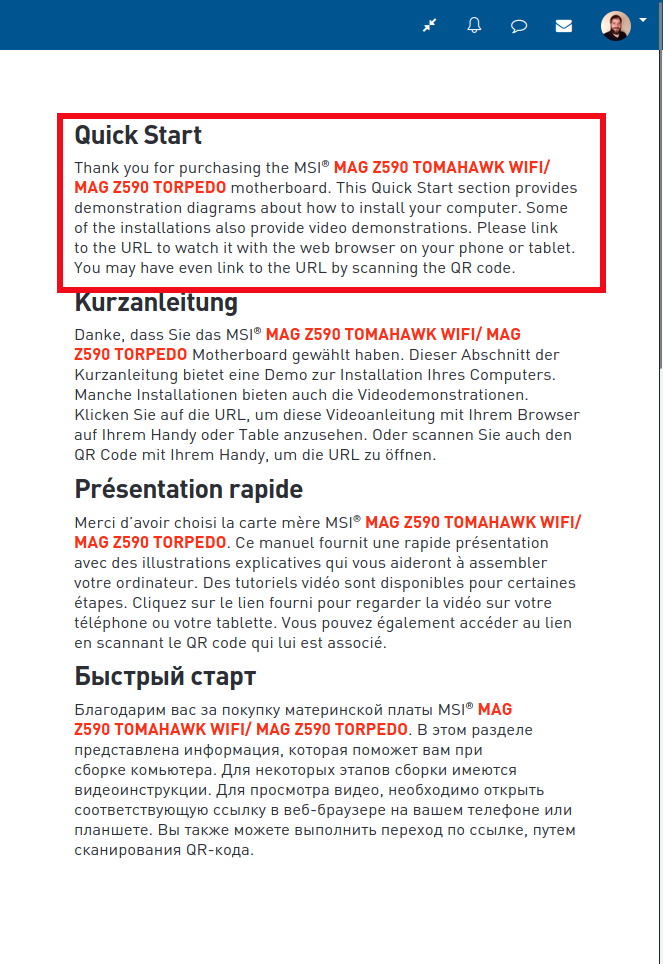
\includegraphics[scale=0.40]{manual-placa.png}
        \caption{Manual placa base MSI MAG Z590 Tomahawk}
    \end{figure}

    \item \textbf{Componentes Placa Base}: a continuación se muestra la imagen superior de la placa base y se indican cada uno de los componentes que se solicitan. La imagen ha sido descargada de la sección ``Galería'' de la página correspondiente a la placa base en la página oficial de MSI. \cite{msi02}

    \begin{figure}[ht]
        \centering
        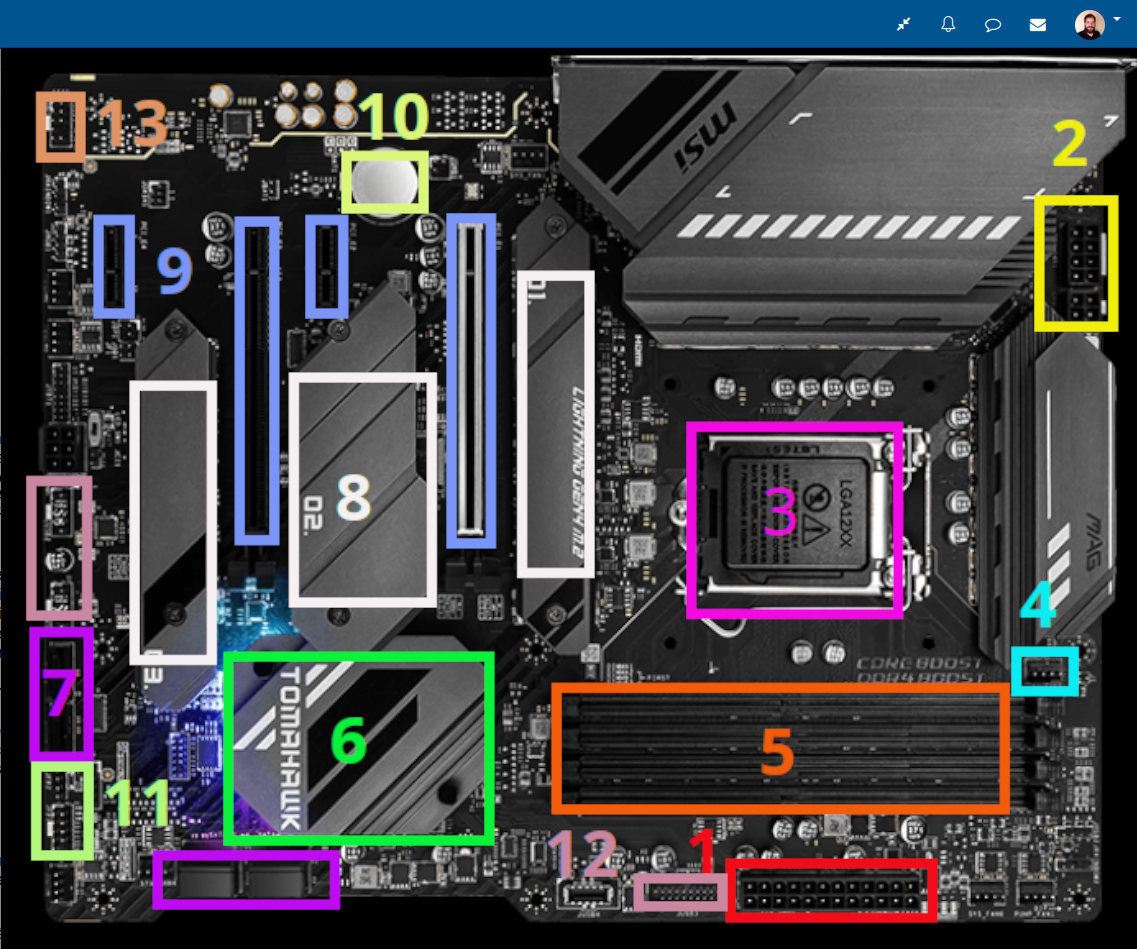
\includegraphics[scale=0.32]{placa-base-tomahawk.png}
        \caption{Vista superior de placa base y conectores}
    \end{figure}

    A continuación se muestra la tabla con todos los componentes señalados en la figura anterior, incluyendo su modelo y función.

    \begin{figure}[ht]
        \centering
        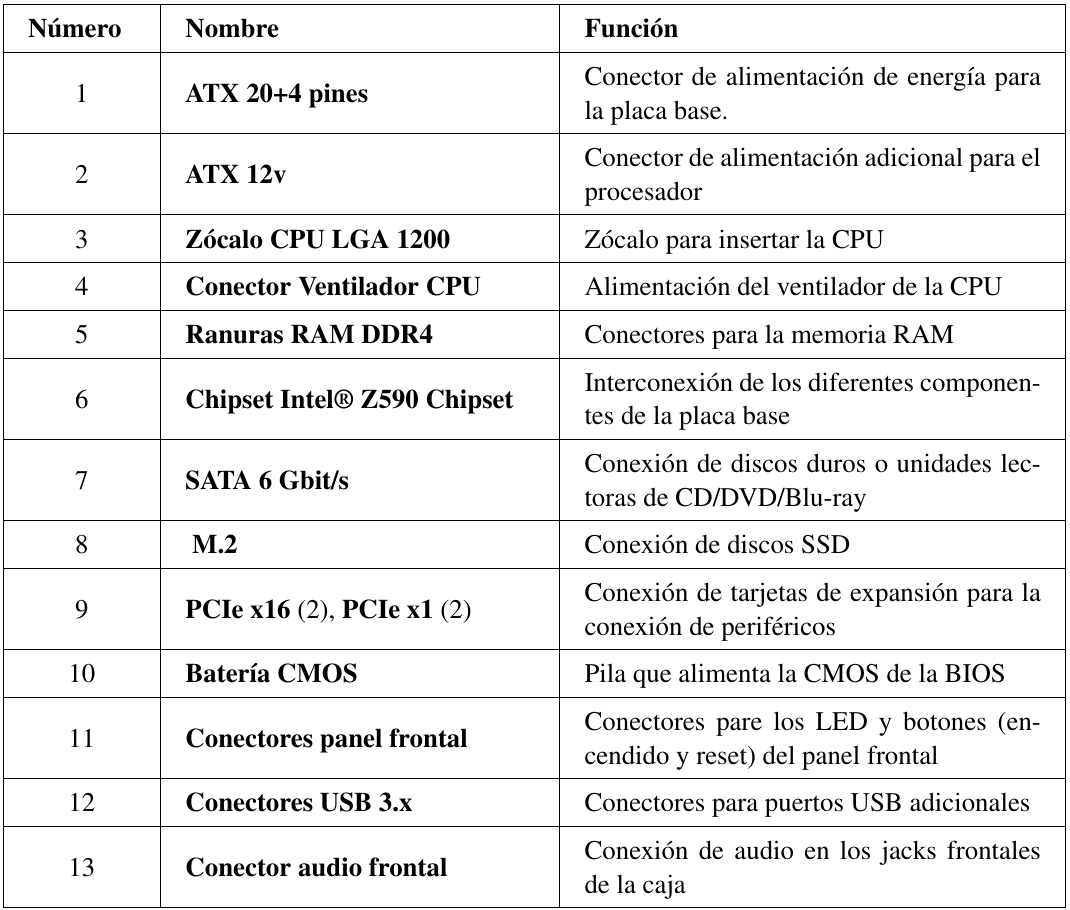
\includegraphics[scale=0.32]{tabla-specs.png}
        \caption{Tabla con las especificaciones de los conectores}
    \end{figure}

    \item \textbf{Panel trasero de la Placa}: por último, mostramos el panel trasero de la placa base, al cual podremos acceder, una vez montada, desde la parte trasera de la caja. Se indican los diferentes tipos de conectores que tiene agrupándolos según su funcionalidad.

\end{enumerate}



% Bibliography

\newpage
\bibliography{citas}
\bibliographystyle{unsrt}

\end{document}